%%%%%%%%%%%%%%%%%%%%%%%%%%%%%%%%%%%%%%%%%%%%%%%%%%%%%%%%%%%%%%%%%%%%%%%%%%%%%%%%%%%%%%%%%%%%%%%%%
%
% Document:      DM  product tree
%
%%%%%%%%%%%%%%%%%%%%%%%%%%%%%%%%%%%%%%%%%%%%%%%%%%%%%%%%%%%%%%%%%%%%%%%%%%%%%%
\documentclass{article}
\usepackage{times,layouts}
\usepackage{tikz,hyperref,amsmath}
\usetikzlibrary{positioning,arrows,shapes,decorations.shapes,shapes.arrows}
\usetikzlibrary{backgrounds,calc}
\usepackage[paperwidth=167.4cm,paperheight=24.648000000000003cm,
left=-2mm,top=3mm,bottom=0mm,right=0mm,
noheadfoot,marginparwidth=0pt,includemp=false,
textwidth=30cm,textheight=50mm]{geometry}
\newcommand\showpage{%
\setlayoutscale{0.5}\setlabelfont{\tiny}\printheadingsfalse\printparametersfalse
\currentpage\pagedesign}
\hypersetup{pdftitle={DM products }, pdfsubject={Diagram illustrating the
products in LSST DM }, pdfauthor={ William O'Mullane}}
\tikzstyle{tbox}=[rectangle,text centered, text width=30mm]
\tikzstyle{wbbox}=[rectangle, rounded corners=3pt, draw=black, top color=blue!50!white, bottom color=white, very thick, minimum height=12mm, inner sep=2pt, text centered, text width=30mm]
\tikzstyle{pbox}=[rectangle, rounded corners=3pt, draw=black, top color=yellow!50!white, bottom color=white, very thick, minimum height=35pt, inner sep=2pt, text centered, text width=35mm]
\tikzstyle{pline}=[-, thick]
\begin{document}
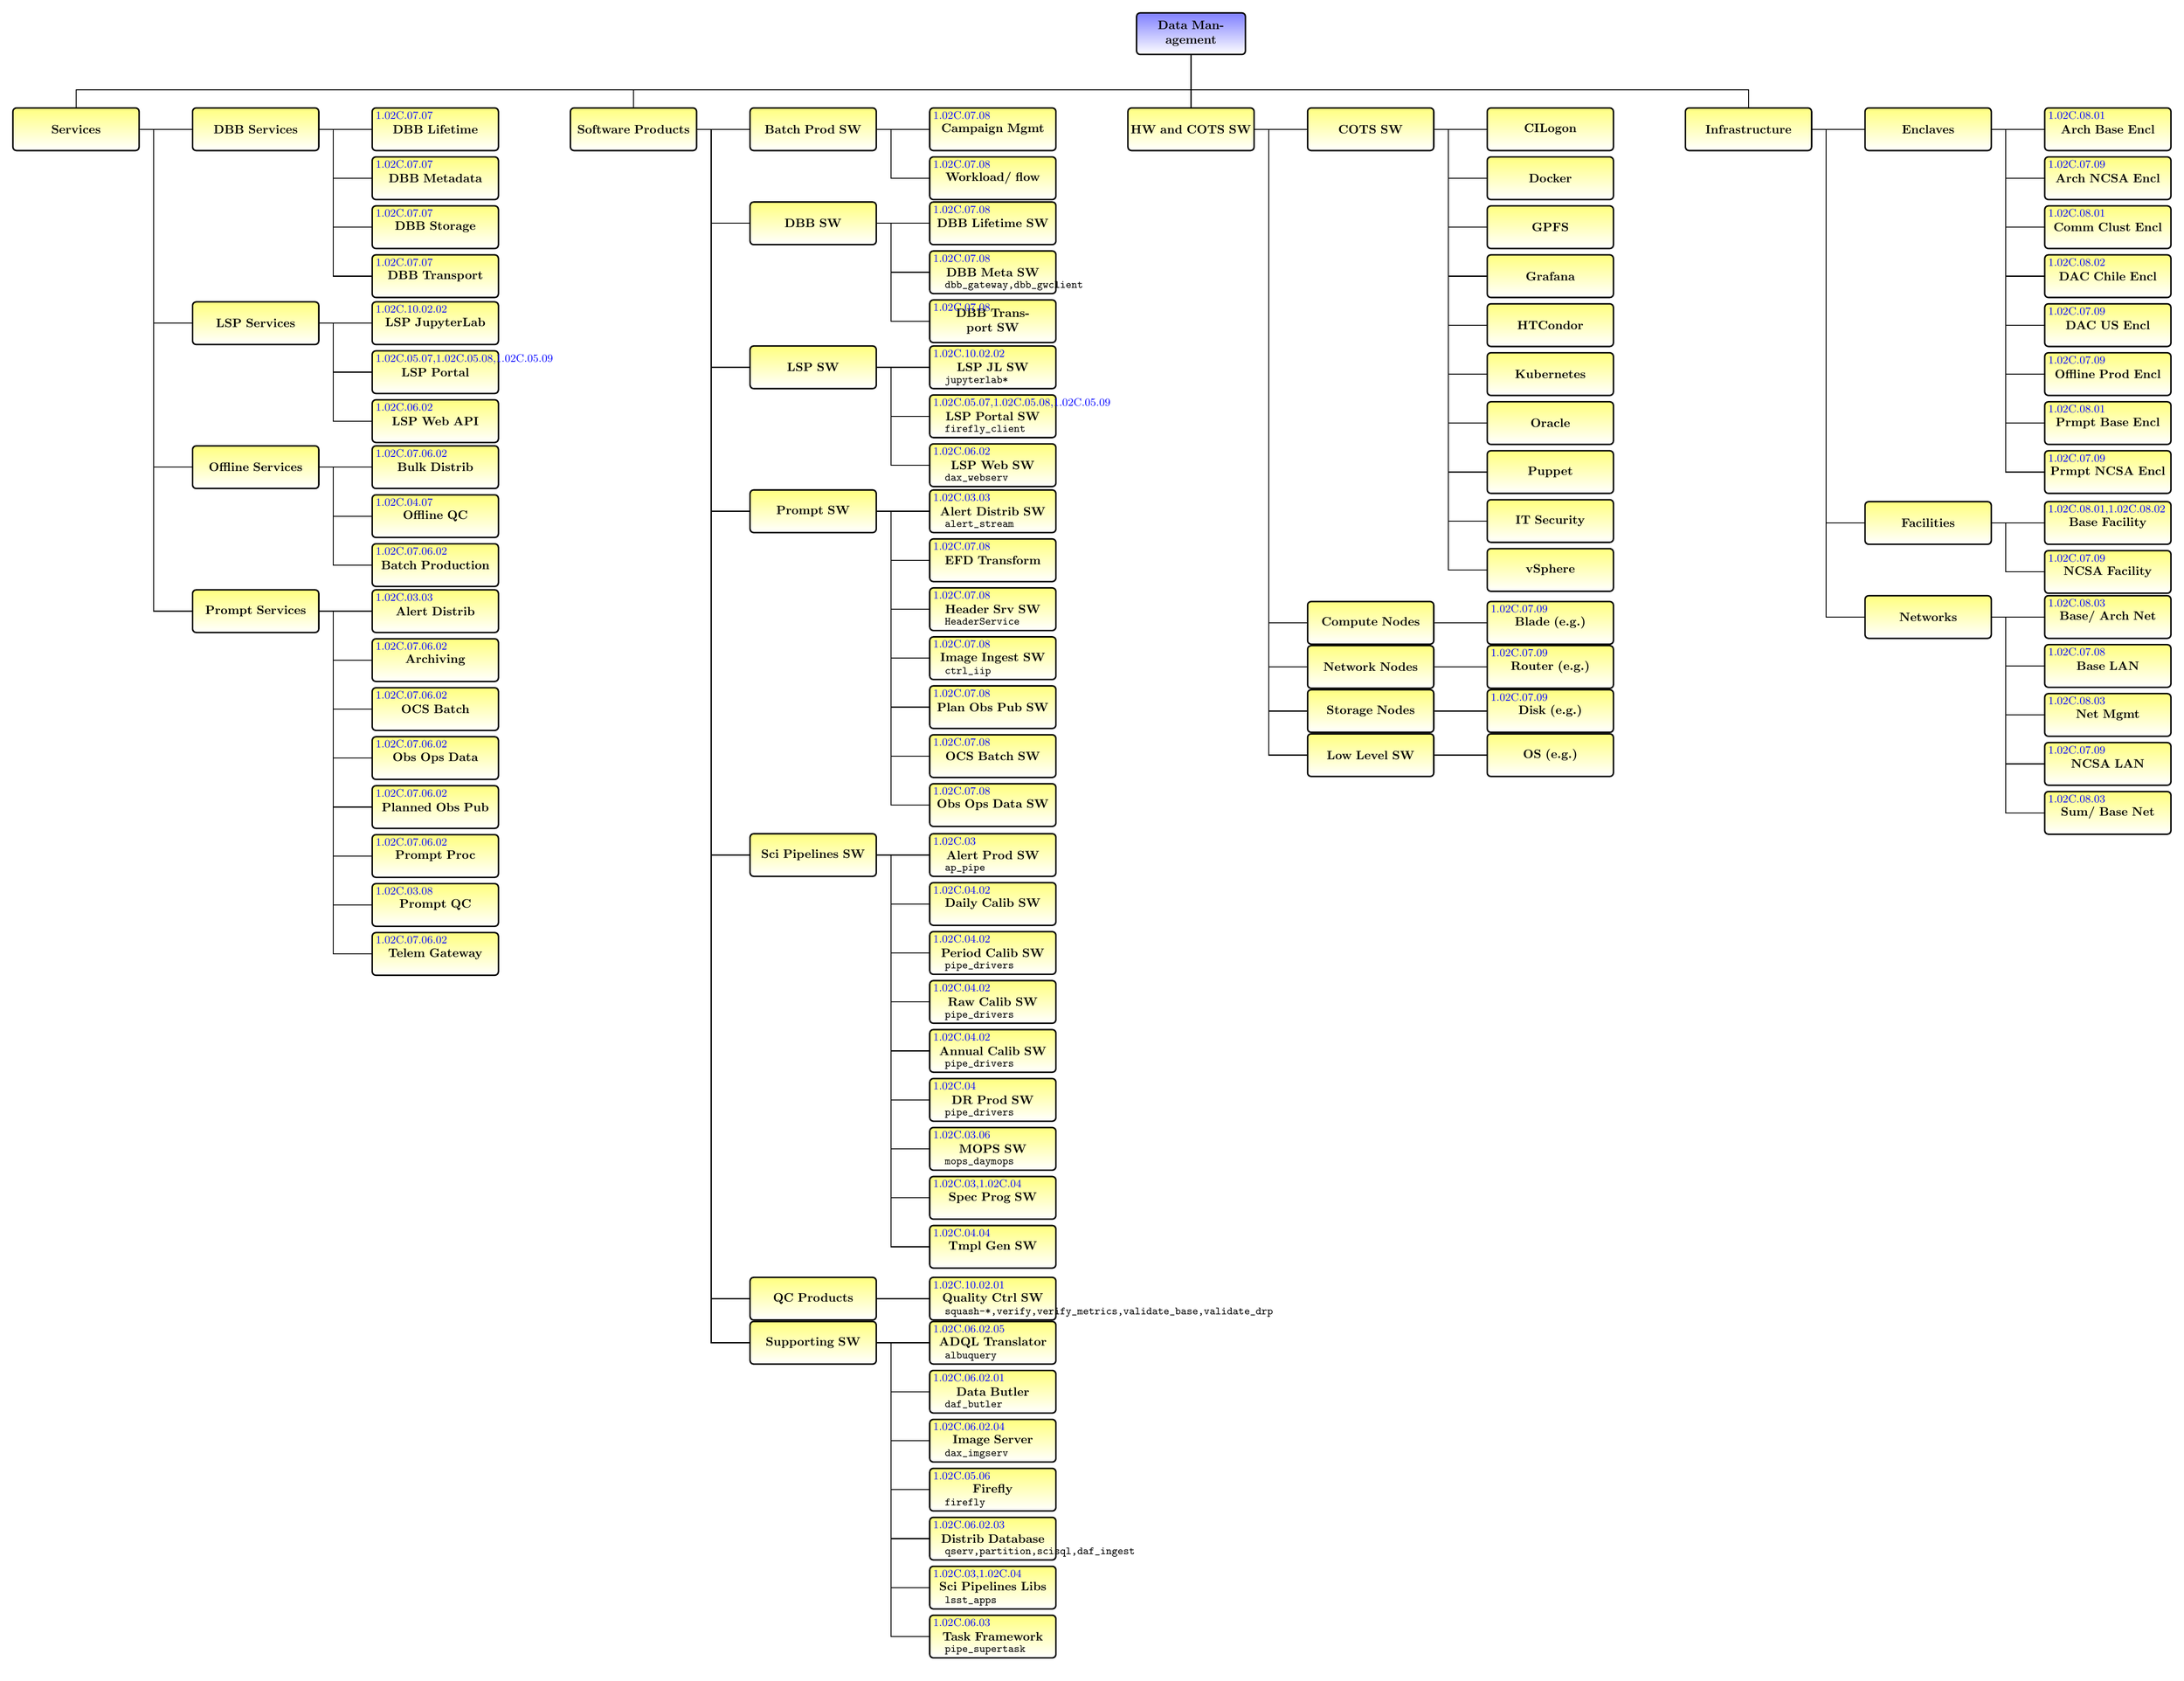
\begin{tikzpicture}[node distance=0mm]
\node (DMSRV) [pbox, 
] {\textbf{Services} };
\node (DBBSRV) [pbox,right=15mm of DMSRV] {\textbf{DBB Services} };
 \draw[pline] (DMSRV.east) -| ++(0.4,0) |- (DBBSRV.west); 
\node (DBBLIFESRV) [pbox,right=15mm of DBBSRV] {\textbf{DBB Lifetime} };
\node [below right] at (DBBLIFESRV.north west) {\small \color{blue}1.02C.07.07} ;
 \draw[pline] (DBBSRV.east) -| ++(0.4,0) |- (DBBLIFESRV.west); 
\node (DBBMDSRV) [pbox,below=4pt of DBBLIFESRV] {\textbf{DBB Metadata} };
\node [below right] at (DBBMDSRV.north west) {\small \color{blue}1.02C.07.07} ;
 \draw[pline] (DBBSRV.east) -| ++(0.4,0) |- (DBBMDSRV.west); 
\node (DBBSTRSRV) [pbox,below=4pt of DBBMDSRV] {\textbf{DBB Storage} };
\node [below right] at (DBBSTRSRV.north west) {\small \color{blue}1.02C.07.07} ;
 \draw[pline] (DBBSRV.east) -| ++(0.4,0) |- (DBBSTRSRV.west); 
\node (DBBTRSRV) [pbox,below=4pt of DBBSTRSRV] {\textbf{DBB Transport} };
\node [below right] at (DBBTRSRV.north west) {\small \color{blue}1.02C.07.07} ;
 \draw[pline] (DBBSRV.east) -| ++(0.4,0) |- (DBBTRSRV.west); 
\node (LSPSRV) [pbox,below=123pt of DBBSRV] {\textbf{LSP Services} };
 \draw[pline] (DMSRV.east) -| ++(0.4,0) |- (LSPSRV.west); 
\node (LSPJLSRV) [pbox,right=15mm of LSPSRV] {\textbf{LSP JupyterLab} };
\node [below right] at (LSPJLSRV.north west) {\small \color{blue}1.02C.10.02.02} ;
 \draw[pline] (LSPSRV.east) -| ++(0.4,0) |- (LSPJLSRV.west); 
\node (LSPPRTLSRV) [pbox,below=4pt of LSPJLSRV] {\textbf{LSP Portal} };
\node [below right] at (LSPPRTLSRV.north west) {\small \color{blue}1.02C.05.07,1.02C.05.08,1.02C.05.09} ;
 \draw[pline] (LSPSRV.east) -| ++(0.4,0) |- (LSPPRTLSRV.west); 
\node (LSPWEBSRV) [pbox,below=4pt of LSPPRTLSRV] {\textbf{LSP Web API} };
\node [below right] at (LSPWEBSRV.north west) {\small \color{blue}1.02C.06.02} ;
 \draw[pline] (LSPSRV.east) -| ++(0.4,0) |- (LSPWEBSRV.west); 
\node (OFFLSRV) [pbox,below=82pt of LSPSRV] {\textbf{Offline Services} };
 \draw[pline] (DMSRV.east) -| ++(0.4,0) |- (OFFLSRV.west); 
\node (BULKDSRV) [pbox,right=15mm of OFFLSRV] {\textbf{Bulk Distrib} };
\node [below right] at (BULKDSRV.north west) {\small \color{blue}1.02C.07.06.02} ;
 \draw[pline] (OFFLSRV.east) -| ++(0.4,0) |- (BULKDSRV.west); 
\node (OFFLQCSRV) [pbox,below=4pt of BULKDSRV] {\textbf{Offline QC} };
\node [below right] at (OFFLQCSRV.north west) {\small \color{blue}1.02C.04.07} ;
 \draw[pline] (OFFLSRV.east) -| ++(0.4,0) |- (OFFLQCSRV.west); 
\node (PRODSRV) [pbox,below=4pt of OFFLQCSRV] {\textbf{Batch Production} };
\node [below right] at (PRODSRV.north west) {\small \color{blue}1.02C.07.06.02} ;
 \draw[pline] (OFFLSRV.east) -| ++(0.4,0) |- (PRODSRV.west); 
\node (PRSRV) [pbox,below=82pt of OFFLSRV] {\textbf{Prompt Services} };
 \draw[pline] (DMSRV.east) -| ++(0.4,0) |- (PRSRV.west); 
\node (ALRTDSTSRV) [pbox,right=15mm of PRSRV] {\textbf{Alert Distrib} };
\node [below right] at (ALRTDSTSRV.north west) {\small \color{blue}1.02C.03.03} ;
 \draw[pline] (PRSRV.east) -| ++(0.4,0) |- (ALRTDSTSRV.west); 
\node (ARCSRV) [pbox,below=4pt of ALRTDSTSRV] {\textbf{Archiving} };
\node [below right] at (ARCSRV.north west) {\small \color{blue}1.02C.07.06.02} ;
 \draw[pline] (PRSRV.east) -| ++(0.4,0) |- (ARCSRV.west); 
\node (OCSBATSRV) [pbox,below=4pt of ARCSRV] {\textbf{OCS Batch} };
\node [below right] at (OCSBATSRV.north west) {\small \color{blue}1.02C.07.06.02} ;
 \draw[pline] (PRSRV.east) -| ++(0.4,0) |- (OCSBATSRV.west); 
\node (OODSSRV) [pbox,below=4pt of OCSBATSRV] {\textbf{Obs Ops Data} };
\node [below right] at (OODSSRV.north west) {\small \color{blue}1.02C.07.06.02} ;
 \draw[pline] (PRSRV.east) -| ++(0.4,0) |- (OODSSRV.west); 
\node (POPSRV) [pbox,below=4pt of OODSSRV] {\textbf{Planned Obs Pub} };
\node [below right] at (POPSRV.north west) {\small \color{blue}1.02C.07.06.02} ;
 \draw[pline] (PRSRV.east) -| ++(0.4,0) |- (POPSRV.west); 
\node (PRPRCSRV) [pbox,below=4pt of POPSRV] {\textbf{Prompt Proc} };
\node [below right] at (PRPRCSRV.north west) {\small \color{blue}1.02C.07.06.02} ;
 \draw[pline] (PRSRV.east) -| ++(0.4,0) |- (PRPRCSRV.west); 
\node (PRQCSRV) [pbox,below=4pt of PRPRCSRV] {\textbf{Prompt QC} };
\node [below right] at (PRQCSRV.north west) {\small \color{blue}1.02C.03.08} ;
 \draw[pline] (PRSRV.east) -| ++(0.4,0) |- (PRQCSRV.west); 
\node (TMGSRV) [pbox,below=4pt of PRQCSRV] {\textbf{Telem Gateway} };
\node [below right] at (TMGSRV.north west) {\small \color{blue}1.02C.07.06.02} ;
 \draw[pline] (PRSRV.east) -| ++(0.4,0) |- (TMGSRV.west); 
\node (DMSW) [pbox, 
right=12.4cm of DMSRV] {\textbf{Software Products} };
\node (BPP) [pbox,right=15mm of DMSW] {\textbf{Batch Prod SW} };
 \draw[pline] (DMSW.east) -| ++(0.4,0) |- (BPP.west); 
\node (CMPGN) [pbox,right=15mm of BPP] {\textbf{Campaign Mgmt} };
\node [below right] at (CMPGN.north west) {\small \color{blue}1.02C.07.08} ;
 \draw[pline] (BPP.east) -| ++(0.4,0) |- (CMPGN.west); 
\node (WLWF) [pbox,below=4pt of CMPGN] {\textbf{Workload/ flow} };
\node [below right] at (WLWF.north west) {\small \color{blue}1.02C.07.08} ;
 \draw[pline] (BPP.east) -| ++(0.4,0) |- (WLWF.west); 
\node (DBB) [pbox,below=41pt of BPP] {\textbf{DBB SW} };
 \draw[pline] (DMSW.east) -| ++(0.4,0) |- (DBB.west); 
\node (DBBLIFE) [pbox,right=15mm of DBB] {\textbf{DBB Lifetime SW} };
\node [below right] at (DBBLIFE.north west) {\small \color{blue}1.02C.07.08} ;
 \draw[pline] (DBB.east) -| ++(0.4,0) |- (DBBLIFE.west); 
\node (DBBMD) [pbox,below=4pt of DBBLIFE] {\textbf{DBB Meta SW} };
\node [below right] at (DBBMD.north west) {\small \color{blue}1.02C.07.08} ;
\node (DBBMDpkg) [tbox,below=3mm of DBBMD.north] {{\small \color{black} \begin{verbatim} dbb_gateway,dbb_gwclient \end{verbatim} }  };
 \draw[pline] (DBB.east) -| ++(0.4,0) |- (DBBMD.west); 
\node (DBBTR) [pbox,below=4pt of DBBMD] {\textbf{DBB Transport SW} };
\node [below right] at (DBBTR.north west) {\small \color{blue}1.02C.07.08} ;
 \draw[pline] (DBB.east) -| ++(0.4,0) |- (DBBTR.west); 
\node (LSP) [pbox,below=82pt of DBB] {\textbf{LSP SW} };
 \draw[pline] (DMSW.east) -| ++(0.4,0) |- (LSP.west); 
\node (LSPJL) [pbox,right=15mm of LSP] {\textbf{LSP JL SW} };
\node [below right] at (LSPJL.north west) {\small \color{blue}1.02C.10.02.02} ;
\node (LSPJLpkg) [tbox,below=3mm of LSPJL.north] {{\small \color{black} \begin{verbatim} jupyterlab* \end{verbatim} }  };
 \draw[pline] (LSP.east) -| ++(0.4,0) |- (LSPJL.west); 
\node (LSPPRTL) [pbox,below=4pt of LSPJL] {\textbf{LSP Portal SW} };
\node [below right] at (LSPPRTL.north west) {\small \color{blue}1.02C.05.07,1.02C.05.08,1.02C.05.09} ;
\node (LSPPRTLpkg) [tbox,below=3mm of LSPPRTL.north] {{\small \color{black} \begin{verbatim} firefly_client \end{verbatim} }  };
 \draw[pline] (LSP.east) -| ++(0.4,0) |- (LSPPRTL.west); 
\node (LSPWEB) [pbox,below=4pt of LSPPRTL] {\textbf{LSP Web SW} };
\node [below right] at (LSPWEB.north west) {\small \color{blue}1.02C.06.02} ;
\node (LSPWEBpkg) [tbox,below=3mm of LSPWEB.north] {{\small \color{black} \begin{verbatim} dax_webserv \end{verbatim} }  };
 \draw[pline] (LSP.east) -| ++(0.4,0) |- (LSPWEB.west); 
\node (PR) [pbox,below=82pt of LSP] {\textbf{Prompt SW} };
 \draw[pline] (DMSW.east) -| ++(0.4,0) |- (PR.west); 
\node (ALRTDSTR) [pbox,right=15mm of PR] {\textbf{Alert Distrib SW} };
\node [below right] at (ALRTDSTR.north west) {\small \color{blue}1.02C.03.03} ;
\node (ALRTDSTRpkg) [tbox,below=3mm of ALRTDSTR.north] {{\small \color{black} \begin{verbatim} alert_stream \end{verbatim} }  };
 \draw[pline] (PR.east) -| ++(0.4,0) |- (ALRTDSTR.west); 
\node (EFDT) [pbox,below=4pt of ALRTDSTR] {\textbf{EFD Transform} };
\node [below right] at (EFDT.north west) {\small \color{blue}1.02C.07.08} ;
 \draw[pline] (PR.east) -| ++(0.4,0) |- (EFDT.west); 
\node (HEADER) [pbox,below=4pt of EFDT] {\textbf{Header Srv SW} };
\node [below right] at (HEADER.north west) {\small \color{blue}1.02C.07.08} ;
\node (HEADERpkg) [tbox,below=3mm of HEADER.north] {{\small \color{black} \begin{verbatim} HeaderService \end{verbatim} }  };
 \draw[pline] (PR.east) -| ++(0.4,0) |- (HEADER.west); 
\node (IIP) [pbox,below=4pt of HEADER] {\textbf{Image Ingest SW} };
\node [below right] at (IIP.north west) {\small \color{blue}1.02C.07.08} ;
\node (IIPpkg) [tbox,below=3mm of IIP.north] {{\small \color{black} \begin{verbatim} ctrl_iip \end{verbatim} }  };
 \draw[pline] (PR.east) -| ++(0.4,0) |- (IIP.west); 
\node (OBSPUB) [pbox,below=4pt of IIP] {\textbf{Plan Obs Pub SW} };
\node [below right] at (OBSPUB.north west) {\small \color{blue}1.02C.07.08} ;
 \draw[pline] (PR.east) -| ++(0.4,0) |- (OBSPUB.west); 
\node (OCSBAT) [pbox,below=4pt of OBSPUB] {\textbf{OCS Batch SW} };
\node [below right] at (OCSBAT.north west) {\small \color{blue}1.02C.07.08} ;
 \draw[pline] (PR.east) -| ++(0.4,0) |- (OCSBAT.west); 
\node (OODS) [pbox,below=4pt of OCSBAT] {\textbf{Obs Ops Data SW} };
\node [below right] at (OODS.north west) {\small \color{blue}1.02C.07.08} ;
 \draw[pline] (PR.east) -| ++(0.4,0) |- (OODS.west); 
\node (PRODN) [pbox,below=246pt of PR] {\textbf{Sci Pipelines SW} };
 \draw[pline] (DMSW.east) -| ++(0.4,0) |- (PRODN.west); 
\node (APPRMPT) [pbox,right=15mm of PRODN] {\textbf{Alert Prod SW} };
\node [below right] at (APPRMPT.north west) {\small \color{blue}1.02C.03} ;
\node (APPRMPTpkg) [tbox,below=3mm of APPRMPT.north] {{\small \color{black} \begin{verbatim} ap_pipe \end{verbatim} }  };
 \draw[pline] (PRODN.east) -| ++(0.4,0) |- (APPRMPT.west); 
\node (CALDAILY) [pbox,below=4pt of APPRMPT] {\textbf{Daily Calib SW} };
\node [below right] at (CALDAILY.north west) {\small \color{blue}1.02C.04.02} ;
 \draw[pline] (PRODN.east) -| ++(0.4,0) |- (CALDAILY.west); 
\node (CALOFFL) [pbox,below=4pt of CALDAILY] {\textbf{Period Calib SW} };
\node [below right] at (CALOFFL.north west) {\small \color{blue}1.02C.04.02} ;
\node (CALOFFLpkg) [tbox,below=3mm of CALOFFL.north] {{\small \color{black} \begin{verbatim} pipe_drivers \end{verbatim} }  };
 \draw[pline] (PRODN.east) -| ++(0.4,0) |- (CALOFFL.west); 
\node (CALPRMPT) [pbox,below=4pt of CALOFFL] {\textbf{Raw Calib SW} };
\node [below right] at (CALPRMPT.north west) {\small \color{blue}1.02C.04.02} ;
\node (CALPRMPTpkg) [tbox,below=3mm of CALPRMPT.north] {{\small \color{black} \begin{verbatim} pipe_drivers \end{verbatim} }  };
 \draw[pline] (PRODN.east) -| ++(0.4,0) |- (CALPRMPT.west); 
\node (CALYEAR) [pbox,below=4pt of CALPRMPT] {\textbf{Annual Calib SW} };
\node [below right] at (CALYEAR.north west) {\small \color{blue}1.02C.04.02} ;
\node (CALYEARpkg) [tbox,below=3mm of CALYEAR.north] {{\small \color{black} \begin{verbatim} pipe_drivers \end{verbatim} }  };
 \draw[pline] (PRODN.east) -| ++(0.4,0) |- (CALYEAR.west); 
\node (DRP) [pbox,below=4pt of CALYEAR] {\textbf{DR Prod SW} };
\node [below right] at (DRP.north west) {\small \color{blue}1.02C.04} ;
\node (DRPpkg) [tbox,below=3mm of DRP.north] {{\small \color{black} \begin{verbatim} pipe_drivers \end{verbatim} }  };
 \draw[pline] (PRODN.east) -| ++(0.4,0) |- (DRP.west); 
\node (MOPS) [pbox,below=4pt of DRP] {\textbf{MOPS SW} };
\node [below right] at (MOPS.north west) {\small \color{blue}1.02C.03.06} ;
\node (MOPSpkg) [tbox,below=3mm of MOPS.north] {{\small \color{black} \begin{verbatim} mops_daymops \end{verbatim} }  };
 \draw[pline] (PRODN.east) -| ++(0.4,0) |- (MOPS.west); 
\node (SP) [pbox,below=4pt of MOPS] {\textbf{Spec Prog SW} };
\node [below right] at (SP.north west) {\small \color{blue}1.02C.03,1.02C.04} ;
 \draw[pline] (PRODN.east) -| ++(0.4,0) |- (SP.west); 
\node (TMPLGEN) [pbox,below=4pt of SP] {\textbf{Tmpl Gen SW} };
\node [below right] at (TMPLGEN.north west) {\small \color{blue}1.02C.04.04} ;
 \draw[pline] (PRODN.east) -| ++(0.4,0) |- (TMPLGEN.west); 
\node (QC) [pbox,below=328pt of PRODN] {\textbf{QC Products} };
 \draw[pline] (DMSW.east) -| ++(0.4,0) |- (QC.west); 
\node (QCSW) [pbox,right=15mm of QC] {\textbf{Quality Ctrl SW} };
\node [below right] at (QCSW.north west) {\small \color{blue}1.02C.10.02.01} ;
\node (QCSWpkg) [tbox,below=3mm of QCSW.north] {{\small \color{black} \begin{verbatim} squash-*,verify,verify_metrics,validate_base,validate_drp \end{verbatim} }  };
 \draw[pline] (QC.east) -| ++(0.4,0) |- (QCSW.west); 
\node (SUPPSW) [pbox,below=0pt of QC] {\textbf{Supporting SW} };
 \draw[pline] (DMSW.east) -| ++(0.4,0) |- (SUPPSW.west); 
\node (ADQL) [pbox,right=15mm of SUPPSW] {\textbf{ADQL Translator} };
\node [below right] at (ADQL.north west) {\small \color{blue}1.02C.06.02.05} ;
\node (ADQLpkg) [tbox,below=3mm of ADQL.north] {{\small \color{black} \begin{verbatim} albuquery \end{verbatim} }  };
 \draw[pline] (SUPPSW.east) -| ++(0.4,0) |- (ADQL.west); 
\node (BUTLER) [pbox,below=4pt of ADQL] {\textbf{Data Butler} };
\node [below right] at (BUTLER.north west) {\small \color{blue}1.02C.06.02.01} ;
\node (BUTLERpkg) [tbox,below=3mm of BUTLER.north] {{\small \color{black} \begin{verbatim} daf_butler \end{verbatim} }  };
 \draw[pline] (SUPPSW.east) -| ++(0.4,0) |- (BUTLER.west); 
\node (DAXIMG) [pbox,below=4pt of BUTLER] {\textbf{Image Server} };
\node [below right] at (DAXIMG.north west) {\small \color{blue}1.02C.06.02.04} ;
\node (DAXIMGpkg) [tbox,below=3mm of DAXIMG.north] {{\small \color{black} \begin{verbatim} dax_imgserv \end{verbatim} }  };
 \draw[pline] (SUPPSW.east) -| ++(0.4,0) |- (DAXIMG.west); 
\node (FIREFLY) [pbox,below=4pt of DAXIMG] {\textbf{Firefly} };
\node [below right] at (FIREFLY.north west) {\small \color{blue}1.02C.05.06} ;
\node (FIREFLYpkg) [tbox,below=3mm of FIREFLY.north] {{\small \color{black} \begin{verbatim} firefly \end{verbatim} }  };
 \draw[pline] (SUPPSW.east) -| ++(0.4,0) |- (FIREFLY.west); 
\node (QSERV) [pbox,below=4pt of FIREFLY] {\textbf{Distrib Database} };
\node [below right] at (QSERV.north west) {\small \color{blue}1.02C.06.02.03} ;
\node (QSERVpkg) [tbox,below=3mm of QSERV.north] {{\small \color{black} \begin{verbatim} qserv,partition,scisql,daf_ingest \end{verbatim} }  };
 \draw[pline] (SUPPSW.east) -| ++(0.4,0) |- (QSERV.west); 
\node (SCIPIPE) [pbox,below=4pt of QSERV] {\textbf{Sci Pipelines Libs} };
\node [below right] at (SCIPIPE.north west) {\small \color{blue}1.02C.03,1.02C.04} ;
\node (SCIPIPEpkg) [tbox,below=3mm of SCIPIPE.north] {{\small \color{black} \begin{verbatim} lsst_apps \end{verbatim} }  };
 \draw[pline] (SUPPSW.east) -| ++(0.4,0) |- (SCIPIPE.west); 
\node (TXF) [pbox,below=4pt of SCIPIPE] {\textbf{Task Framework} };
\node [below right] at (TXF.north west) {\small \color{blue}1.02C.06.03} ;
\node (TXFpkg) [tbox,below=3mm of TXF.north] {{\small \color{black} \begin{verbatim} pipe_supertask \end{verbatim} }  };
 \draw[pline] (SUPPSW.east) -| ++(0.4,0) |- (TXF.west); 
\node (HWCOTS) [pbox, 
right=12.4cm of DMSW] {\textbf{HW and COTS SW} };
\node (COTS) [pbox,right=15mm of HWCOTS] {\textbf{COTS SW} };
 \draw[pline] (HWCOTS.east) -| ++(0.4,0) |- (COTS.west); 
\node (CILOGON) [pbox,right=15mm of COTS] {\textbf{CILogon} };
 \draw[pline] (COTS.east) -| ++(0.4,0) |- (CILOGON.west); 
\node (DOCKER) [pbox,below=4pt of CILOGON] {\textbf{Docker} };
 \draw[pline] (COTS.east) -| ++(0.4,0) |- (DOCKER.west); 
\node (GPFS) [pbox,below=4pt of DOCKER] {\textbf{GPFS} };
 \draw[pline] (COTS.east) -| ++(0.4,0) |- (GPFS.west); 
\node (GRAFANA) [pbox,below=4pt of GPFS] {\textbf{Grafana} };
 \draw[pline] (COTS.east) -| ++(0.4,0) |- (GRAFANA.west); 
\node (HTCONDOR) [pbox,below=4pt of GRAFANA] {\textbf{HTCondor} };
 \draw[pline] (COTS.east) -| ++(0.4,0) |- (HTCONDOR.west); 
\node (K8S) [pbox,below=4pt of HTCONDOR] {\textbf{Kubernetes} };
 \draw[pline] (COTS.east) -| ++(0.4,0) |- (K8S.west); 
\node (ORACLE) [pbox,below=4pt of K8S] {\textbf{Oracle} };
 \draw[pline] (COTS.east) -| ++(0.4,0) |- (ORACLE.west); 
\node (PUPPET) [pbox,below=4pt of ORACLE] {\textbf{Puppet} };
 \draw[pline] (COTS.east) -| ++(0.4,0) |- (PUPPET.west); 
\node (SECURITY) [pbox,below=4pt of PUPPET] {\textbf{IT Security} };
 \draw[pline] (COTS.east) -| ++(0.4,0) |- (SECURITY.west); 
\node (VSPHERE) [pbox,below=4pt of SECURITY] {\textbf{vSphere} };
 \draw[pline] (COTS.east) -| ++(0.4,0) |- (VSPHERE.west); 
\node (HWCOMP) [pbox,below=369pt of COTS] {\textbf{Compute Nodes} };
 \draw[pline] (HWCOTS.east) -| ++(0.4,0) |- (HWCOMP.west); 
\node (DELL8) [pbox,right=15mm of HWCOMP] {\textbf{Blade (e.g.)} };
\node [below right] at (DELL8.north west) {\small \color{blue}1.02C.07.09} ;
 \draw[pline] (HWCOMP.east) -| ++(0.4,0) |- (DELL8.west); 
\node (HWNET) [pbox,below=0pt of HWCOMP] {\textbf{Network Nodes} };
 \draw[pline] (HWCOTS.east) -| ++(0.4,0) |- (HWNET.west); 
\node (NETX) [pbox,right=15mm of HWNET] {\textbf{Router (e.g.)} };
\node [below right] at (NETX.north west) {\small \color{blue}1.02C.07.09} ;
 \draw[pline] (HWNET.east) -| ++(0.4,0) |- (NETX.west); 
\node (HWSTOR) [pbox,below=0pt of HWNET] {\textbf{Storage Nodes} };
 \draw[pline] (HWCOTS.east) -| ++(0.4,0) |- (HWSTOR.west); 
\node (SAN2) [pbox,right=15mm of HWSTOR] {\textbf{Disk (e.g.)} };
\node [below right] at (SAN2.north west) {\small \color{blue}1.02C.07.09} ;
 \draw[pline] (HWSTOR.east) -| ++(0.4,0) |- (SAN2.west); 
\node (LLSW) [pbox,below=0pt of HWSTOR] {\textbf{Low Level SW} };
 \draw[pline] (HWCOTS.east) -| ++(0.4,0) |- (LLSW.west); 
\node (CENTOS) [pbox,right=15mm of LLSW] {\textbf{OS (e.g.)} };
 \draw[pline] (LLSW.east) -| ++(0.4,0) |- (CENTOS.west); 
\node (INFRA) [pbox, 
right=12.4cm of HWCOTS] {\textbf{Infrastructure} };
\node (ENC) [pbox,right=15mm of INFRA] {\textbf{Enclaves} };
 \draw[pline] (INFRA.east) -| ++(0.4,0) |- (ENC.west); 
\node (ENCARCB) [pbox,right=15mm of ENC] {\textbf{Arch Base Encl} };
\node [below right] at (ENCARCB.north west) {\small \color{blue}1.02C.08.01} ;
 \draw[pline] (ENC.east) -| ++(0.4,0) |- (ENCARCB.west); 
\node (ENCARCN) [pbox,below=4pt of ENCARCB] {\textbf{Arch NCSA Encl} };
\node [below right] at (ENCARCN.north west) {\small \color{blue}1.02C.07.09} ;
 \draw[pline] (ENC.east) -| ++(0.4,0) |- (ENCARCN.west); 
\node (ENCCOMM) [pbox,below=4pt of ENCARCN] {\textbf{Comm Clust Encl} };
\node [below right] at (ENCCOMM.north west) {\small \color{blue}1.02C.08.01} ;
 \draw[pline] (ENC.east) -| ++(0.4,0) |- (ENCCOMM.west); 
\node (ENCDACC) [pbox,below=4pt of ENCCOMM] {\textbf{DAC Chile Encl} };
\node [below right] at (ENCDACC.north west) {\small \color{blue}1.02C.08.02} ;
 \draw[pline] (ENC.east) -| ++(0.4,0) |- (ENCDACC.west); 
\node (ENCDACU) [pbox,below=4pt of ENCDACC] {\textbf{DAC US Encl} };
\node [below right] at (ENCDACU.north west) {\small \color{blue}1.02C.07.09} ;
 \draw[pline] (ENC.east) -| ++(0.4,0) |- (ENCDACU.west); 
\node (ENCOFFL) [pbox,below=4pt of ENCDACU] {\textbf{Offline Prod Encl} };
\node [below right] at (ENCOFFL.north west) {\small \color{blue}1.02C.07.09} ;
 \draw[pline] (ENC.east) -| ++(0.4,0) |- (ENCOFFL.west); 
\node (ENCPRB) [pbox,below=4pt of ENCOFFL] {\textbf{Prmpt Base Encl} };
\node [below right] at (ENCPRB.north west) {\small \color{blue}1.02C.08.01} ;
 \draw[pline] (ENC.east) -| ++(0.4,0) |- (ENCPRB.west); 
\node (ENCPRN) [pbox,below=4pt of ENCPRB] {\textbf{Prmpt NCSA Encl} };
\node [below right] at (ENCPRN.north west) {\small \color{blue}1.02C.07.09} ;
 \draw[pline] (ENC.east) -| ++(0.4,0) |- (ENCPRN.west); 
\node (FAC) [pbox,below=287pt of ENC] {\textbf{Facilities} };
 \draw[pline] (INFRA.east) -| ++(0.4,0) |- (FAC.west); 
\node (FACBASE) [pbox,right=15mm of FAC] {\textbf{Base Facility} };
\node [below right] at (FACBASE.north west) {\small \color{blue}1.02C.08.01,1.02C.08.02} ;
 \draw[pline] (FAC.east) -| ++(0.4,0) |- (FACBASE.west); 
\node (FACNCSA) [pbox,below=4pt of FACBASE] {\textbf{NCSA Facility} };
\node [below right] at (FACNCSA.north west) {\small \color{blue}1.02C.07.09} ;
 \draw[pline] (FAC.east) -| ++(0.4,0) |- (FACNCSA.west); 
\node (NET) [pbox,below=41pt of FAC] {\textbf{Networks} };
 \draw[pline] (INFRA.east) -| ++(0.4,0) |- (NET.west); 
\node (NETBA) [pbox,right=15mm of NET] {\textbf{Base/ Arch Net} };
\node [below right] at (NETBA.north west) {\small \color{blue}1.02C.08.03} ;
 \draw[pline] (NET.east) -| ++(0.4,0) |- (NETBA.west); 
\node (NETBASE) [pbox,below=4pt of NETBA] {\textbf{Base LAN} };
\node [below right] at (NETBASE.north west) {\small \color{blue}1.02C.07.08} ;
 \draw[pline] (NET.east) -| ++(0.4,0) |- (NETBASE.west); 
\node (NETMGMT) [pbox,below=4pt of NETBASE] {\textbf{Net Mgmt} };
\node [below right] at (NETMGMT.north west) {\small \color{blue}1.02C.08.03} ;
 \draw[pline] (NET.east) -| ++(0.4,0) |- (NETMGMT.west); 
\node (NETNCSA) [pbox,below=4pt of NETMGMT] {\textbf{NCSA LAN} };
\node [below right] at (NETNCSA.north west) {\small \color{blue}1.02C.07.09} ;
 \draw[pline] (NET.east) -| ++(0.4,0) |- (NETNCSA.west); 
\node (NETSB) [pbox,below=4pt of NETNCSA] {\textbf{Sum/ Base Net} };
\node [below right] at (NETSB.north west) {\small \color{blue}1.02C.08.03} ;
 \draw[pline] (NET.east) -| ++(0.4,0) |- (NETSB.west); 
\node (DM) [wbbox, above=15mm of HWCOTS]{\textbf{Data Management}};
 \draw[pline]   (DMSRV.north) -- ++(0.0,0.5) -| (DM.south) ; 
 \draw[pline]   (DMSW.north) -- ++(0.0,0.5) -| (DM.south) ; 
 \draw[pline]   (HWCOTS.north) -- ++(0.0,0.5) -| (DM.south) ; 
 \draw[pline]   (INFRA.north) -- ++(0.0,0.5) -| (DM.south) ; 
\end{tikzpicture}
\end{document}
